\documentclass[11pt]{extarticle}
\usepackage[margin=1.27cm]{geometry}
\usepackage{setspace}
\usepackage{fontspec}
% \usepackage[T1]{fontenc}
% \usepackage[utf8]{inputenc}
\usepackage{amsmath,txfonts,amssymb,nicefrac,mathtools,pifont} %for math
\usepackage{array,tabularx,multirow,fmtcount} %for tables
\usepackage{tikz, pgfplots} %for diagram
\usepackage{multicol} %for multiple column
\usepackage{enumerate,enumitem,adjustbox} %for ordered list
\usepackage{graphicx,subcaption,wrapfig,tcolorbox} %for figure
\usepackage{xparse} %for commands & environments
\usepackage{lipsum} %miscellaneous
\usepackage{colortbl,xcolor,soul} %for default table & border

% #ANCHOR Font settings
\setmainfont{Oxygen}
\newfontfamily\banglafont[Script=Bengali]{Baloo Da 2}
\newfontfamily{\lstsansserif}{IBM Plex Mono}
\renewcommand{\normalsize}{\fontsize{11.5pt}{13pt}\selectfont}


\setlength{\arrayrulewidth}{0.35 pt}
\definecolor{border}{HTML}{A1A1AA}
\arrayrulecolor{border}


% #ANCHOR Document settings
\linespread{1.45}
\setlength\parindent{0pt}
\setlength\parskip{16pt}
\setlist[enumerate]{noitemsep}
\usetikzlibrary{shapes.geometric,decorations.pathreplacing,trees,arrows,positioning,shapes,fit,calc,decorations.markings, decorations.text}
\tikzset{every node/.append style={font=\footnotesize}}
\usepgfplotslibrary{fillbetween}
\pgfdeclarelayer{background}
\pgfsetlayers{background,main}
\pgfplotsset{compat=1.18}
\columnseprule=1pt
\everymath{\displaystyle}
% #ANCHOR Hypernation
\tolerance=1
\emergencystretch=\maxdimen
\hyphenpenalty=10000
\hbadness=10000
\newlength{\colWidth}



% #ANCHOR Colors
\definecolor{azure(colorwheel)}{rgb}{0.0, 0.5, 1.0}
\definecolor{carminepink}{rgb}{0.92, 0.3, 0.26}
\definecolor{orange}{rgb}{0.9, 0.55, 0.22}
\definecolor{violet}{rgb}{0.60, 0.45, 1}
% Syantax Highlighting Colors
\definecolor{keyword}{HTML}{D73A4A}
\definecolor{number}{HTML}{015CC5}
\definecolor{comment}{HTML}{6A737D}
\definecolor{string}{HTML}{1D825E}
\definecolor{function}{HTML}{743FD1}
\definecolor{orange}{HTML}{CF7842}
\definecolor{codeblack}{HTML}{24292F}
\definecolor{divider}{HTML}{A1A1AA}
\definecolor{border}{HTML}{D1D1D1}


% #ANCHOR Ordered & Unordered List
\setlist[itemize,1]{left=0cm, label={\textbullet}}
\setlist[itemize,2,3,4,5,6,7,8,9,10]{left=0.6cm, label={\textbullet}}
\setlist[enumerate,1]{left=0cm}
\setlist[enumerate,2,3,4,5,6,7,8,9,10]{left=0.6cm}
\setul{0.5ex}{0.125ex}



% #ANCHOR Colored Box
\let\oldul\ul
\renewcommand{\ul}[2][keyword]{\text{\setulcolor{#1}\oldul{#2}}}
\newcommand{\redbox}[1]{%
{\color{red}\fbox{\color{black}#1}}
}
\newcommand{\red}[1]{%
\textcolor{red}{#1}
}
\newcommand{\redeq}[1]{%
\text{\color{red}$#1$}
}
\newcommand{\mred}[1]{%
\textcolor{keyword}{#1}
}
\newcommand{\mredeq}[1]{%
\textcolor{keyword}{$#1$}
}
\newcommand{\blue}[1]{%
% {\color{number}#1\hspace{-0.4ex}}
\textcolor{number}{#1}
}
\newcommand{\blueeq}[1]{%
\text{\color{number}$#1$}
}
\newcommand{\cyanbox}[1]{%
{\color{teal}\fbox{\textcolor{black}{#1}}}
}
\newcommand{\cyan}[1]{%
\textcolor{teal}{#1}
}
\newcommand{\pink}[1]{%
\textcolor{magenta}{#1}
}
\newcommand{\orange}[1]{%
\textcolor{orange}{#1}
}
\newcommand{\violet}[1]{%
{\color{violet}#1}
}
\newcommand{\cyaneq}[1]{%
\text{\color{teal}$#1$}
}
\newcommand{\gray}[1]{%
\textcolor{comment}{#1}
}
\newcommand{\pinkeq}[1]{%
\text{\color{magenta}$#1$}
}
\renewcommand{\columnseprulecolor}{\color{divider}}




% #ANCHOR Tabular commands
\newcolumntype{P}[1]{>{\centering\arraybackslash}p{#1}}
\newcolumntype{M}[1]{>{\centering\arraybackslash}m{#1}}
\newcolumntype{C}{>{\centering\arraybackslash}X}
\newcommand{\rspan}[2]{\multirow{#1}{*}{#2}}
\newcommand{\thc}[1]{%
\multicolumn{1}{|c|}{\textbf{#1}}
}
\newcommand{\thcx}[1]{%
\multicolumn{1}{|C|}{\textbf{#1}}
}
\newcommand{\thl}[1]{%
\multicolumn{1}{|l|}{\textbf{#1}}
}
\newcommand{\thr}[1]{%
\multicolumn{1}{|r|}{\textbf{#1}}
}
% Adjusting arraystretch to modify vertical padding
\renewcommand{\arraystretch}{1.25}
% Adjusting tabcolsep to modify horizontal padding
\setlength{\tabcolsep}{10pt}



% #ANCHOR Math commands
\newcommand{\set}[1]{\{$#1$\}}
\newcommand{\tabs}{\ \ \ \ \ \ }
\newcommand{\tab}{\ \ \ }
\newcommand{\cmark}{\ding{51}}%
\newcommand{\xmark}{\ding{55}}%
\newcommand{\boldi}[1]{\boldsymbol{#1}}%
\newcommand{\wspace}{\ \ = \ \ }



% #ANCHOR New commands
\newcommand{\Title}[1]{%
   \begin{center}
      \textbf{\Large{#1}}
   \end{center}
}
\newcommand{\Heading}[1]{%
   \par\vspace{\dimexpr -\baselineskip + 16pt}
   {\fontsize{12pt}{13pt}\selectfont\textbf{#1}}
   \par\vspace{\dimexpr -\baselineskip + 6pt}
}
\newcommand{\BuleHeading}[1]{%
   \par\vspace{\dimexpr -\baselineskip + 16pt}
   {\fontsize{12pt}{13pt}\selectfont\textbf{\textcolor{number}{#1}}}
   \par\vspace{\dimexpr -\baselineskip + 6pt}
}
\newcommand{\CHeading}[1]{%
   \par\vspace{\dimexpr -\baselineskip + 16pt}
   \hspace{\fill}
   {\fontsize{12pt}{13pt}\selectfont\textbf{#1}}
   \hspace{\fill}
   \par\vspace{\dimexpr -\baselineskip + 6pt}
}
\newcommand{\Section}[1]{%
   \par\vspace{\dimexpr -\baselineskip + 16pt}
   \hspace{\fill}
   {\fontsize{13pt}{13pt}\selectfont\textbf{#1}}
   \hspace{\fill}
   \par\vspace{\dimexpr -\baselineskip + 6pt}
}
\newcommand{\seteqno}[1]{%
   \ \cdots \ \cdots \ \cdots \ (#1)
}
\newcommand{\eqor}{%
   \Rightarrow \ \ 
}
\newcommand{\tsub}[1]{%
\textsubscript{#1}\hspace{-0.45ex}
}
\newcommand{\tsup}[1]{%
\textsuperscript{#1}\hspace{-0.45ex}
}
\newcommand{\cbox}[2][cyan]{
\tikz\node[draw=#1,circle,inner sep=2pt,baseline=(a.base)](a){#2};
}
\newcommand{\hrline}{%
\vspace{1ex} {\color{gray}\hrule} \vspace{4ex}
}
\newcommand{\divideX}[1][divider]{{\hspace{1ex}\color{#1}{\vrule}\hspace{1ex}}}
\newcommand{\Reference}[2][Reference]{

\vspace{-0.5\baselineskip}
\begin{center}
   {\fontspec{Merriweather}\textbf{#1:} \textit{#2}} 
\end{center}
}
\newcommand{\bn}[1]{%
   {\banglafont #1}
}

\NewDocumentCommand{\Column}{O{0.49} O{1.5em} m m}{
   \setlength{\colWidth}{\linewidth-#1\linewidth-#2}
   \begin{minipage}[t]{#1\linewidth}
      \noindent
         #3
      \end{minipage}\hspace{\fill}{\color{divider}\vrule width 0.35pt}\hspace{\fill}
      \begin{minipage}[t]{\colWidth}
      \noindent
         #4
   \end{minipage}
}

% Vector commands
\renewcommand{\vec}[1]{\underline{\,\mathrm{#1}}}
\renewcommand{\r}{\mathrm{\textbf{r}}}
\renewcommand{\v}{\mathrm{v}}
\renewcommand{\a}{\mathrm{a}}
\newcommand{\dx}{{\,dx}}
\newcommand{\dy}{{\,dy}}
\newcommand{\dz}{{\,dz}}
\newcommand{\dr}{{\,d\vec{r}}}
\newcommand{\dtheta}{{\,d\theta}}
\newcommand{\dphi}{{\,d\phi}}
\newcommand{\drho}{{\,d\rho}}
\let\oldkappa\kappa
\renewcommand{\kappa}{\scalebox{1.25}{$\oldkappa$}}
\newcommand{\vf}[2][t]{\vec{#2}(#1)}
\newcommand{\norm}[1]{\left\lVert\ #1\ \right\rVert}
\newcommand{\osint}[1][]{\oint\displaylimits_\mathrm{#1}}
\newcommand{\sint}[1][]{\int\displaylimits_\mathrm{#1}}
\newcommand{\mint}{\int\displaylimits}
\newcommand{\miint}{\iint\displaylimits}
\newcommand{\miiint}{\iiint\displaylimits}


\NewDocumentCommand{\dt}{O{t} m}{\vec{#2}^\prime(#1)}
\NewDocumentCommand{\vdt}{m}{\vec{#1}^\prime}
\NewDocumentCommand{\dtt}{O{t} m}{\vec{#2}^{\prime\prime}(#1)}
\NewDocumentCommand{\vdtt}{m}{\vec{#1}^{\prime\prime}}
\NewDocumentCommand{\vecf}{O{x} O{y} O{z}}{#1 \ \vec{i} + #2 \ \vec{j} + #3 \ \vec{k}}
\NewDocumentCommand{\vecxy}{O{x} O{y}}{#1 \ \vec{i} + #2 \ \vec{j}}
\NewDocumentCommand{\vecbf}{O{x} O{y} O{z}}{\left(#1,\ #2,\ #3\right)}

\begin{document}
\Title{Line, Double, Triple Integral}

\Section{\cyan{Line Integral}}
\textbf{\mred{15(b)}} Calculate the
work done when a force $\vec{F}=3xy\vec{i}-y^2\vec{j}$ moves a particle in the $xy$ plane from $(0,0)$ to $(1,2)$ along the parabola $y=2x^2$.

\Heading{Solution:}
\begin{minipage}[t]{0.69\linewidth}
\noindent
   Work done $ = \oint \mathrm{F. \ \dr}$\\[1ex]
   \begin{tabular}{lll}
      $\therefore \oint \mathrm{F. \ \dr}$
      & $= \oint  3xy\dx-y^2\dy$
      & \multirow{3}{*}{\hspace{3ex}\divideX$\begin{aligned}
         \text{but, \ } y=2x^2\\
         \therefore dy = 4x\dx
      \end{aligned}$}\\
      & $\begin{aligned}
         &= \int_{0}^{1} 3x \cdot 2x^2 \dx - \left(2x^2\right)^2 4x\dx\\[1ex]
         &= \int_{0}^{1} \left(6x^3 - 16x^5\right)\dx\\[1ex]
         &= \left[\frac{6x^4}{4}-\frac{16x^6}{6}\right]_{0}^{1}\\[1ex]
         &= \frac{6}{4}-\frac{16}{6}\\[1ex]
         &= -\frac{7}{6}
      \end{aligned}$
   \end{tabular}
\end{minipage}\hspace{0.5ex}{\color{divider}\vrule width 0.35pt}\hspace{0.5ex}
\begin{minipage}[t]{0.29\linewidth}
\noindent
   Given that,\\
   $\begin{aligned}
      &\vec{F} = 3xy\vec{i}-y^2\vec{j}\\
      &\vec{r} = x\vec{i}+y\vec{j}\\
      \therefore \ & \dr = \dx\vec{i}+\dy\vec{j}\\
      \therefore \ & \mathrm{F. \dr} = 3xy\dx-y^2\dy\\
   \end{aligned}$
\end{minipage}


\textbf{\mred{10(b)}} Evaluate$\oint(x^2y^2\dx-xy^3\dy)$ where $C$ is the triangle with vertices $(0,0),\ (1,0),\ (1,1)$.

\Heading{Concept:}
\begin{multicols}{2}
   \begin{center}
      Clockwise direction\\[2ex]
      \begin{tikzpicture}[decoration={markings,mark=at position 0.5 with {\arrow{angle 90}}}]
         \draw[-triangle 45] (0,-1) -- (0,3);
         \draw[-triangle 45] (-1,0) -- (3,0);
   
         \coordinate (O) at (0,0);
         \coordinate (A) at (2.5,0);
         \coordinate (B) at (2.5,2);
   
         \draw[postaction={decorate}] (O) -- (B);
         \draw[postaction={decorate}] (B) -- (A);
         \draw[postaction={decorate}] (A) -- (O);
   
         \node[below left] at (O) {$(0,0)\ O$};
         \node[below right] at (A) {$A\ (1,0)$};
         \node[right] at (B) {$B\ (1,1)$};
      \end{tikzpicture}
   
      $\osint[OBAO] = \sint[OB] \tab+\sint[BA] \tab+\sint[AO]$
   \end{center}

   \columnbreak
   \begin{center}
      Anti-Clockwise direction\\[2ex]
      \begin{tikzpicture}[decoration={markings,mark=at position 0.5 with {\arrow{angle 90}}}]
         \draw[-triangle 45] (0,-1) -- (0,3);
         \draw[-triangle 45] (-1,0) -- (3,0);
   
         \coordinate (O) at (0,0);
         \coordinate (A) at (2.5,0);
         \coordinate (B) at (2.5,2);
   
         \draw[postaction={decorate}] (O) -- (A);
         \draw[postaction={decorate}] (A) -- (B);
         \draw[postaction={decorate}] (B) -- (O);
   
         \node[below left] at (O) {$(0,0)\ O$};
         \node[below right] at (A) {$A\ (1,0)$};
         \node[right] at (B) {$B\ (1,1)$};
      \end{tikzpicture}
   
      
      $\osint[OABO] = \sint[OA] \tab+\sint[AB] \tab+\sint[BO]$
   \end{center}
\end{multicols}


\begin{center}
   \begin{tabular}{lll}
      $\mathrm{OA},\ \mathrm{AO}$
      &$y=0$
      &$\therefore \dy=0$\\
      $\mathrm{AB},\ \mathrm{BA}$
      &$x=1$
      &$\therefore \dx=0$\\
      $\mathrm{BO},\ \mathrm{OB}$
      &$x=y$
      &$\therefore \dx=\dy$\\
   \end{tabular}
\end{center}
 
\pagebreak
\Heading{Solution:}
\begin{tabular}{ll}
   $\begin{aligned}
      & \osint[OABO] x^2 y^2 \dx - xy^3 \dy\\
      & = \sint[\substack{OA\\[0.5ex]y=0\\[0.5ex]dy=0}]
      x^2 y^2 \dx - xy^3 \dy
      + \sint[\substack{AB\\[0.5ex]x=1\\[0.5ex]dx=0}]
      x^2 y^2 \dx - xy^3 \dy
      + \sint[\substack{BO\\[0.5ex]x=y\\[0.5ex]dx=dy}]
      x^2 y^2 \dx - xy^3 \dy\\[0.5ex]
      & =\int 0+\int_0^1 0-1 \cdot y^3 \dy+\int_1^{0} x^4\dx - x^4\dx\\[0.5ex]
      & =0-\left[\frac{y^4}{4}\right]_0^1+0 \\[1ex]
      & =-\left(\frac{1}{4}-0\right) \\[1ex]
      & =-\frac{1}{4}
   \end{aligned}$
      &
   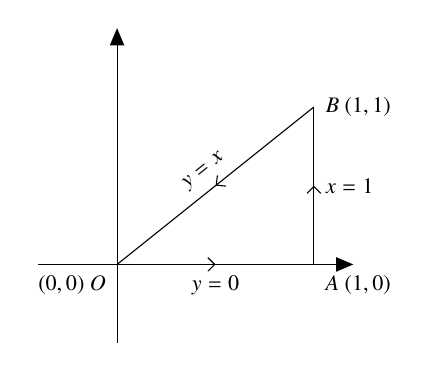
\begin{tikzpicture}[decoration={markings,mark=at position 0.5 with {\arrow{angle 90}}}]
      \draw[-triangle 45] (0,-1) -- (0,3);
      \draw[-triangle 45] (-1,0) -- (3,0);
   
      \coordinate (O) at (0,0);
      \coordinate (A) at (2.5,0);
      \coordinate (B) at (2.5,2);
   
      \draw[postaction={decorate}] (O) -- (A)
      node [below, midway] {$y=0$};
      \draw[postaction={decorate}] (A) -- (B)
      node [right, midway] {$x=1$};
      \draw[postaction={decorate}] (B) -- (O)
      node [above, midway, sloped] {$y=x$};
   
      \node[below left] at (O) {$(0,0)\ O$};
      \node[below right] at (A) {$A\ (1,0)$};
      \node[right] at (B) {$B\ (1,1)$};
   \end{tikzpicture}
\end{tabular}


\vspace{5ex}
\textbf{\mred{\#}} Evaluate$\oint\left(xy-x^2\right)\dx+x^2y\dy$ \ where $C$ is the triangle bounded by the line $y=0,\ x=1,\ y=x$.
\Heading{Solution:}
\begin{tabular}{ll}
   $\begin{aligned}
      & \osint[C]\left(xy-x^2\right)\dx+x^2y\dy\\
      & = \sint[OA] \ \ C \tabs\tabs + \sint[AB]
      \ \ C \tabs\tabs + \sint[BO] \ \ C \tabs\tabs\\[0.5ex]
      & = \sint[\substack{OA\\[0.5ex]y=0\\[0.5ex]dy=0}]
      (0-x^2)\dx+0
      + \sint[\substack{AB\\[0.5ex]x=1\\[0.5ex]dx=0}]
      0+1^2 y\dy
      + \sint[\substack{BO\\[0.5ex]x=y\\[0.5ex]dx=dy}]
      (x^2-x^2)\dx+x^3\dx\\[0.5ex]
      & =\int_0^1 -x^2\dx +\int_0^1 y\dy + \int_1^{0} x^3\dx\\[1ex]
      & =\left[\frac{-x^3}{3}\right]_0^1+\left[\frac{y^2}{2}\right]_0^1+\left[\frac{x^4}{4}\right]_1^0 \\[1ex]
      & =\left(-\frac{1}{3}-0\right) + 
      \left(\frac{1}{2}-0\right) + 
      \left(0-\frac{1}{4}\right)\\[1ex]
      & =-\frac{1}{3}+\frac{1}{2}-\frac{1}{4} \tab = -\frac{1}{12}
   \end{aligned}$
      &
   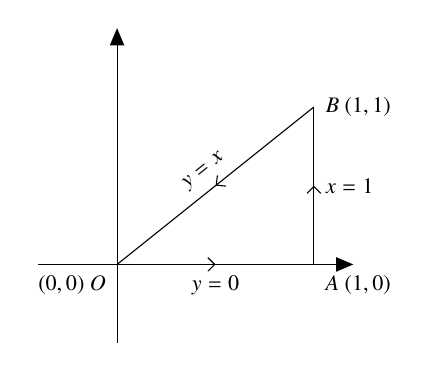
\begin{tikzpicture}[decoration={markings,mark=at position 0.5 with {\arrow{angle 90}}}]
      \draw[-triangle 45] (0,-1) -- (0,3);
      \draw[-triangle 45] (-1,0) -- (3,0);
   
      \coordinate (O) at (0,0);
      \coordinate (A) at (2.5,0);
      \coordinate (B) at (2.5,2);
   
      \draw[postaction={decorate}] (O) -- (A)
      node [below, midway] {$y=0$};
      \draw[postaction={decorate}] (A) -- (B)
      node [right, midway] {$x=1$};
      \draw[postaction={decorate}] (B) -- (O)
      node [above, midway, sloped] {$y=x$};
   
      \node[below left] at (O) {$(0,0)\ O$};
      \node[below right] at (A) {$A\ (1,0)$};
      \node[right] at (B) {$B\ (1,1)$};
   \end{tikzpicture}
\end{tabular}

\pagebreak
\textbf{\mred{10(a)}} If the vector field is given by $\vec{F}=(2x-y+z)\vec{i} + (x+y-z^2)\vec{j} + (3x-2y+4z)\vec{k}$, evaluate the line integral over a circular path given by $x^2+y^2=16,\ z=0$.

\Heading{Solution:}

Since \ $z=0$, \ \ $\therefore \vec{F}=(2x-y)\vec{i} + (x+y)\vec{j} + (3x-2y)\vec{k}$

\begin{tabularx}{\textwidth}{Xp{5cm}}
   \begin{adjustbox}{valign=t}
      $\begin{aligned}
         & \text{Here, }\\
         &\vec{r} = x\vec{i}+y\vec{j}+0\vec{k}\\
         \therefore \ & \dr = \dx\vec{i}+\dy\vec{j}+0\vec{k}\\
         \therefore \ & \mathrm{F. \dr} = (2x-y)\dx+(x+y)\dy\\
      \end{aligned}$
   \end{adjustbox}
   &
   \begin{adjustbox}{valign=t}
      % \divideX
      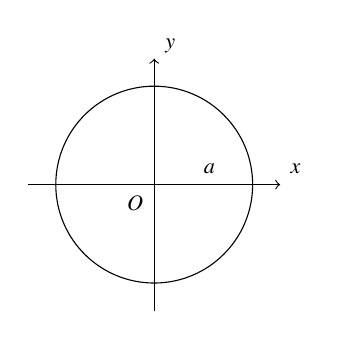
\begin{tikzpicture}
         \draw (0,0) circle (1.25cm);
         \draw[->] (0,-1.6) -- (0,1.6);
         \draw[->] (-1.6,0) -- (1.6,0);
         \node[below left] at (0,0) {$O$};
         \node[above] at (0.7,0) {$a$};
         \node[below right] at (0,2) {$y$};
         \node[above left] at (2,0) {$x$};
      \end{tikzpicture} 
   \end{adjustbox}
\end{tabularx}


\begin{tabular}{ll}
   Now, & \divideX\tabs Parametric equation of a circle,\\
   \begin{adjustbox}{valign=t}
      $\begin{aligned}
         & \text { Line integral } = \oint \mathrm{F. \ \dr}\\[1ex]
         & =\int_0^{2\pi} (2a\cos\theta-a\sin\theta)(-a\sin\theta\dtheta) + (a\cos\theta+a\sin\theta)(a\cos\theta\dtheta)
      \end{aligned}$
   \end{adjustbox}
   &
   \divideX
   \begin{adjustbox}{valign=t}
      $\begin{aligned}
         x &= a\cos\theta
         \text{\tab \ \ and \tab}
         y = a\sin\theta \\
         \therefore \dx &= -a\sin\theta
         \text{\tab and \tab}
         \therefore \dy = a\cos\theta\\
         & 0 \leq \theta \leq 2\pi\\
      \end{aligned}$
   \end{adjustbox}
\end{tabular}

$\begin{aligned}
   & =\int_0^{2\pi} \left[-2 a^2 \sin \theta \cos \theta+{a^2 \sin ^2 \theta} + {a^2 \cos^2 \theta}+a^2 \sin \theta \cos \theta\right]\dtheta\\[1ex]
   & =\int_0^{2\pi} \left[a^2 \left(\sin ^2 \theta + \cos^2 \theta\right)-2 a^2 \sin \theta \cos \theta+a^2 \sin \theta \cos \theta\right]\dtheta\\[1ex]
   & =\int_0^{2\pi} a^2 - a^2 \sin \theta \cos \theta\dtheta
   \quad =\int_0^{2\pi} a^2 \left(1 - \sin\theta\cos\theta\right)\dtheta\\[1ex]
   & = a^2 \int_0^{2\pi} \left(1 - \frac{\sin2\theta}{2}\right)\dtheta
   \quad = a^2 \int_0^{2\pi} \left(1 - \frac{1}{2}\sin2\theta\right)\dtheta\\[1ex]
   & = a^2 \ \left[\theta + \frac{1}{2}\cos2\theta\cdot\frac{1}{2}\right]_0^{2\pi} 
   \quad = a^2 \ \left[\theta + \frac{1}{4}\cos2\theta\right]_0^{2\pi}\\[1ex]
   & = a^2 \ \left(\left(2\pi + \frac{1}{4} \ \cos4\pi\right)-\left(0 + \frac{1}{4} \ \cos0\right)\right)\\[1ex]
   & = a^2 \ \left(2\pi + \frac{1}{4}\cdot 1-0 - \frac{1}{4}\cdot 1\right)\\
   & = 2\pi a^2
\end{aligned}$


\pagebreak
\textbf{\mred{17}} Evaluate the integral $\miint_R xy\dx\dy$ where $R$ is the 1st quadrant of the circle $x^2+y^2=a^2$

\Heading{Solution:}
\begin{minipage}[t]{0.66\linewidth}
\noindent
   \begin{adjustbox}{valign=t}
      $\begin{aligned}
         & \miint_R xy\dx\dy = \mint_{x=0}^a \mint_{y=0}^{\sqrt{a^2-x^2}} xy \dy\dx  \\[1ex]
         & =\int_0^a x \cdot \left[\frac{y^2}{2}\right]_0^{\sqrt{a^2-x^2}} \dx
         \tab =\int_0^a x  \cdot \frac{1}{2}\left(a^2-x^2\right) \dx
         \tab =\frac{1}{2} \int_0^a \left(a^2x-x^3\right) \dx \\[1.5ex]
         & =\frac{1}{2}\left[\frac{a^2 x^2}{2}-\frac{x^4}{4}\right]_0^a
         \tab =\frac{1}{2}\left[\frac{a^4}{2}-\frac{a^4}{4}\right]
         \tab =\frac{1}{2}\left[\frac{2 a^4-a^4}{4}\right]=\frac{a^4}{8}
      \end{aligned}$
   \end{adjustbox}
\end{minipage}\hspace{0.5ex}{\color{divider}\vrule width 0.35pt}\hspace{0.5ex}
\begin{minipage}[t]{0.32\linewidth}
\noindent
   \begin{adjustbox}{valign=t}
      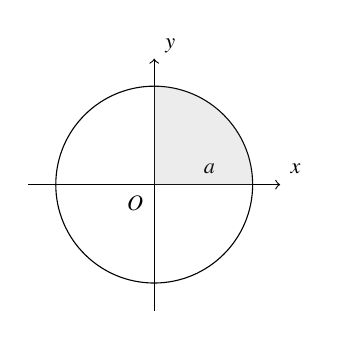
\begin{tikzpicture}
         \draw (0,0) circle (1.25cm);
         \draw[->] (0,-1.6) -- (0,1.6);
         \draw[->] (-1.6,0) -- (1.6,0);
         
         \node[below left] at (0,0) {$O$};
         \node[above] at (0.7,0) {$a$};
         \node[below right] at (0,2) {$y$};
         \node[above left] at (2,0) {$x$};
      
         \clip (0,0) circle (1.25cm);
         \begin{scope}
            \fill[gray,opacity=0.15] (0,0) rectangle (1.5,1.5);
         \end{scope}
      \end{tikzpicture}
   \end{adjustbox}
   \begin{tabular}{ll}
      $\begin{aligned}
         & \text{Given that, }\\
         & x^2+y^2=a^2 \\
         \therefore \ & y^2=a^2-x^2 \\
         \therefore \ & y= \pm \sqrt{a^2-x^2}\\
      \end{aligned}$
      &
      \hspace{0.5em}
      $\begin{aligned}
         & \text {and, } \\
         & x^2=a^2 \\
         & \therefore x= \pm a
      \end{aligned}$
   \end{tabular}
\end{minipage}


\vspace{4ex}
\textbf{\mred{17}} Evaluate the integral $\miint_R xy\dx\dy$ where $R$ is the 3rd quadrant of the circle $x^2+y^2=a^2$

\Heading{Solution:}
\begin{minipage}[t]{0.68\linewidth}
\noindent
   \begin{adjustbox}{valign=t}
      $\begin{aligned}
         & \miint_R xy\dx\dy = \mint_{x=-a}^0 \mint_{y=-\sqrt{a^2-x^2}}^{0} xy \dy\dx  \\[1ex]
         & =\int^0_{-a} x \cdot \left[\frac{y^2}{2}\right]^0_{\sqrt{a^2-x^2}} \dx
         \tab =\int^0_{-a} x  \cdot -\frac{1}{2}\left(a^2-x^2\right) \dx
         \tab =-\frac{1}{2} \int^0_{-a} \left(a^2x-x^3\right) \dx \\[1.5ex]
         & =-\frac{1}{2}\left[\frac{a^2 x^2}{2}-\frac{x^4}{4}\right]^0_{-a}
         \tab =-\frac{1}{2}\left[\frac{a^4}{2}-\frac{a^4}{4}\right]
         \tab =-\frac{1}{2}\left[\frac{2 a^4-a^4}{4}\right]=-\frac{a^4}{8}
      \end{aligned}$
   \end{adjustbox}
\end{minipage}\hspace{0.5ex}{\color{divider}\vrule width 0.35pt}\hspace{0.5ex}
\begin{minipage}[t]{0.3\linewidth}
\noindent
   \begin{adjustbox}{valign=t}
      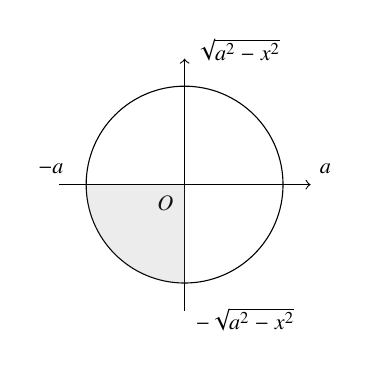
\begin{tikzpicture}
         \draw (0,0) circle (1.25cm);
         \draw[->] (0,-1.6) -- (0,1.6);
         \draw[->] (-1.6,0) -- (1.6,0);
         
         \node[below left] at (0,0) {$O$};
         % \node[above] at (0.7,0) {$a$};
         \node[below right] at (0,2) {$\sqrt{a^2-x^2}$};
         \node[above right] at (0,-2) {$-\sqrt{a^2-x^2}$};
         \node[above left] at (2,0) {$a$};
         \node[above right] at (-2,0) {$-a$};
      
         \clip (0,0) circle (1.25cm);
         \begin{scope}
            \fill[gray,opacity=0.15] (0,0) rectangle (-1.5,-1.5);
         \end{scope}
      \end{tikzpicture}
   \end{adjustbox}
   \begin{tabular}{ll}
      $\begin{aligned}
         & \text{Given that, }\\
         & x^2+y^2=a^2 \\
         \therefore \ & y^2=a^2-x^2 \\
         \therefore \ & y= \pm \sqrt{a^2-x^2}\\
      \end{aligned}$
      &
      \hspace{0.5em}
      $\begin{aligned}
         & \text {and, } \\
         & x^2=a^2 \\
         & \therefore x= \pm a
      \end{aligned}$
   \end{tabular}
\end{minipage}

\pagebreak


\vspace{4ex}
\textbf{\mred{\#}} Calculate the volume of the solid bounded by the surface $x=0,\ y=0,\ x+y+z=1$ and $z=0$
\Heading{Solution:}
\begin{tabularx}{\textwidth}{Xp{6.4cm}}
   \begin{adjustbox}{valign=t}
      $\begin{aligned}
         \text {Volume }
         & = \int_{x=0}^1 \int_{y=0}^{1-x}
         \int_0^{1-x-y} \dz\dy\dx\\[0.5ex]
         & = \int_{x=0}^1 \int_{y=0}^{1-x}\left[z\right]_0^{1-x-y} \dy\dx \\[0.5ex]
         & =\int_{x=0}^1 \int_{y=0}^{1-x}\left(1-x-y\right) \dy\dx \\[0.5ex]
         & =\int_{x=0}^1\left[y-x y-\frac{y^2}{2}\right]_0^{1-x} \dx \\[0.5ex]
         & =\int_0^1\left[1-x-x\left(1-x\right)-\frac{1}{2}\left(1-x\right)^2\right] \dx \\[0.5ex]
         & =\int_0^1\left[1-x-x+x^2-\frac{1}{2}\left(1^2-2.1.x+x^2\right)\right] \dx \\[0.5ex]
         & =\int_0^1\left[1-2x+x^2-\frac{1}{2}+x-\frac{1}{2}x^2\right] \dx \\[0.5ex]
         & =\int_0^1\left[\frac{1}{2}-x+\frac{1}{2}x^2\right] \dx 
         \quad =\left[\frac{1}{2}x-\frac{x^2}{2}+\frac{1}{2}\frac{x^3}{3}\right]_0^1 \\[0.5ex]
         &= \frac{1}{2}-\frac{1}{2}+\frac{1}{2}\cdot\frac{1}{3} \tab = \frac{1}{6} \\[0.5ex]
      \end{aligned}$
   \end{adjustbox}
   &
   \divideX
   \begin{adjustbox}{valign=t}
      $\begin{aligned}
         & \text { Give that } \\
         & x+y+z=1 \\
         & \Rightarrow z=1-x-y \\
         & \text { and } x+y=1 \\
         & \Rightarrow y=1-x \\
         & \text { and also } \\
         & x=1 \\
      \end{aligned}$
   \end{adjustbox}
\end{tabularx}

\pagebreak
\textbf{\mred{\#}} Evaluate $\miint_R \left(x^2+y^2\right)\dx\dy$ \ throughout the area enclosed by the curves $y=4x,\ x+y=3,\ y=0$ and $y=2$.

\begin{tabularx}{\textwidth}{Xp{7cm}}
   \begin{adjustbox}{valign=t}
      $\begin{aligned}
         \text{Area } &=\miint_R \left(x^2+y^2\right)\dx\dy\\
         & =\int_{y=0}^{2}  \int_{x=\frac{y}{4}}^{3-y} \left(x^2+y^2\right)\dx\dy\\[1ex]
         & =\int_{y=0}^{2} \left[\frac{x^3}{3}+xy^2\right]_{x=\frac{y}{4}}^{3-y}\dy\\[1ex]
         & =\int_{y=0}^{2} \left[
            \left(\frac{(3-y)^3}{3}+(3-y)\ y^2\right)-
            \left(\frac{\left(\frac{y}{4}\right)^3}{3}+\left(\frac{y}{4}\right)\ y^2\right)
            \right]\dy\\[1ex]
         & =\int_{y=0}^{2} \left[
            \frac{1}{3}
            (3-y)^3+(3y^2-y^3)\ -
            \frac{y^3}{4^3.\ 3}-\frac{y^3}{4}
            \right]\dy\\[1ex]
         & =\left[
            \frac{1}{3}\cdot -\frac{(3-y)^4}{4}
            +\frac{3y^3}{3}-\frac{y^4}{4}\ -
            \frac{1}{4^3.\ 3}\frac{y^4}{4}
            -\frac{1}{4}\frac{y^4}{4}
            \right]_{y=0}^{2}\\[1ex]
         & =\left[
            \frac{1}{3}\cdot -\frac{(3-2)^4}{4}
            +\frac{3.\ 2^3}{3}-\frac{2^4}{4}\ -
            \frac{1}{4^3.\ 3}\frac{2^4}{4}
            -\frac{1}{4}\frac{2^4}{4}
            \right]\\[1ex]
         & =-\frac{1}{12}+8-4-\frac{1}{48}-1+\frac{81}{12}\\[1ex]
         & = \frac{463}{48} \tab \mathrm{sq.\ unit\ area}
      \end{aligned}$
   \end{adjustbox}
   &
   \begin{adjustbox}{valign=t}
      \divideX
      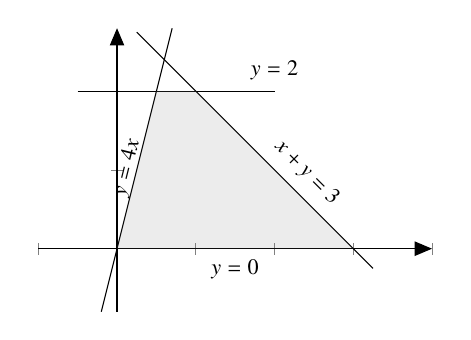
\begin{tikzpicture}
         \begin{axis}[
            x=1cm, y=1cm,
            xmin=-1, xmax=4,
            axis lines=middle,axis line style={-triangle 45},  
            xticklabels={}, yticklabels={},clip=false, no markers]
            \addplot[domain=-0.2:0.7, name path=A]{4*x}
            node[above=-4pt, midway, sloped] {$y=4x$};
            \addplot[domain=0.25:3.25, name path=B]{3-x}
            node[above right, midway, sloped] {$x+y=3$};
            \addplot[domain=-0.5:3.5, name path=Y]{0}
            node[below, midway] {$y=0$};
            \addplot[domain=-0.5:2, name path=X]{2}
            node[above] {$y=2$};
      
            \path[name intersections={of=A and X,by=AX}];
            \path[name intersections={of=X and B,by=XB}];
            \path[name intersections={of=B and Y,by=BY}];
            \path[name intersections={of=Y and A,by=YA}];
      
            \fill[gray,opacity=0.15] (AX) -- (XB) -- (BY) -- (YA) -- cycle;
         \end{axis}
      \end{tikzpicture}
   \end{adjustbox}
\end{tabularx}

\vspace{5ex}
\textbf{\mred{\#}} Use double integral to find the area bounded by $x+2y-4=0$ and $2y=16-x^2$



\Heading{Solution:}
\begin{minipage}[t]{0.66\linewidth}
   \noindent
   \begin{adjustbox}{valign=t}
      $\begin{aligned}
         & \text{Given that }\\
         & x+2y-4=0 \tabs \Rightarrow \ 2y = 4-x \tabs 
         \Rightarrow \  y = \frac{4-x}{2} \seteqno{i} \\[-0.5ex]
         & \text{Put }\ x=0, \ \therefore y=2
         \text{\tabs and \tabs Put }\ y=0 \ \therefore x=4\\[2ex]
         & 2y=16-x^2 \tabs \Rightarrow \  y = 8-\frac{1}{2}x^2 \seteqno{ii}\\[-0.5ex]
         & \text{Put }\ x=0, \ \therefore y=8\\[2ex]
         & \text{Solving equation } (i) \text{ and } (ii),\\
         & 4-x = 16-x^2 \ \Rightarrow \  x^2-x-12=0 \ \Rightarrow \  (x-4)(x+3) = 0 \ \therefore \ x=-3,4
      \end{aligned}$
      \divideX
   \end{adjustbox}
\end{minipage}
\begin{minipage}[t]{0.32\linewidth}
\noindent
   \begin{adjustbox}{valign=t}
      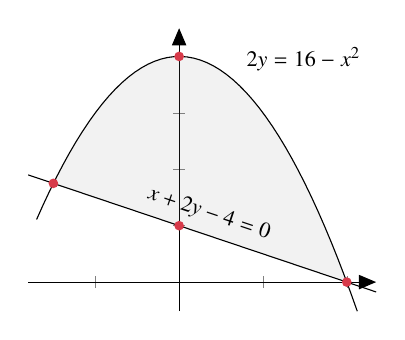
\begin{tikzpicture}
         \begin{axis}[axis lines=middle,axis line style={-triangle 45}, ymax = 9, xticklabels={}, yticklabels={}, width=6cm, clip=false]
            \addplot[domain=-3.4:4.25, samples=50, name path=curve]{(16-x^2)/2} node[above right,midway] {$2y=16-x^2$};
            \addplot[domain=-3.6:4.7, name path=line]{2-x/2}
            node[above, midway, sloped] {$x+2y-4=0$};
            \addplot[gray,opacity=0.1] fill between[of=curve and line, soft clip={domain=-3:4}];

            \fill[keyword](0,2) circle (1.75pt);
            \fill[keyword](4,0) circle (1.75pt);
            \fill[keyword](0,8) circle (1.75pt);
            \fill[keyword](-3,3.5) circle (1.75pt);
         \end{axis}
      \end{tikzpicture}
   \end{adjustbox}
\end{minipage}

\vspace{1.5ex}
$\begin{aligned}
   \therefore\text{Area} = \miint_{R} \dx\dy
   &= \int_{-3}^{4} \int_{y=2-\frac{x}{2}}^{8-\frac{x^2}{2}}  \dy\dx\\[1ex]
   &= \int_{-3}^{4} \left[y\right]_{y=2-\frac{x}{2}}^{8-\frac{x^2}{2}} \dx\\[1ex]
   &= \int_{-3}^{4} \left(8-\frac{x^2}{2}-2+\frac{x}{2}\right) \dx\\[1ex]
   &= \left[8x-\frac{x^3}{2.3}-2x+\frac{x^2}{2.2}\right]_{-3}^{4} 
   = \left[6x-\frac{x^3}{6}+\frac{x^2}{4}\right]_{-3}^{4}\\[1ex]
   &= \left(6.4-\frac{4^3}{6}+\frac{4^2}{4}\right)-
   \left(6.(-3)-\frac{(-3)^3}{6}+\frac{(-3)^2}{4}\right)\\[1ex]
   &= 24-\frac{64}{6}+4+18-\frac{27}{6}+\frac{9}{4}\\[1ex]
   &= \frac{343}{12} \tab \mathrm{sq.\ unit\ area}
\end{aligned}$

\vspace{4ex}
\textbf{\mred{12}} Evaluate the followings:\\[1ex]
\begin{tabular}{lll}
   $(i) \ \mint_{0}^{\frac{\pi}{2}} \mint_{0}^{\frac{\pi}{2}} \mint_{0}^1 \rho^3 \sin \phi \cos \phi \drho \dphi \dtheta$
   &\hspace{1em}
   $(ii) \ \mint_1^{3} \mint_x^{x^2} \mint_0^{lnz} x e^y \dy\dz\dx$
\end{tabular}

\vspace{2ex}
\Heading{Solution $(i)$:}
$\begin{aligned}
& =\mint_{\theta=0}^{\frac{\pi}{2}} \mint_{\phi=0}^{\frac{\pi}{2}}\left[\frac{\rho^4}{4}\right]_0^1 \sin \phi \cos \phi \dphi \dtheta \quad 
= \mint_{\theta=0}^{\frac{\pi}{2}} \mint_{\phi=0}^{\frac{\pi}{2}} \frac{1}{4} \cdot \frac{\sin 2 \phi}{2} \dphi \dtheta \quad
= \mint_{\theta=0}^{\frac{\pi}{2}} \frac{1}{8}\left[\frac{-\cos 2 \phi}{2}\right]_0^{\frac{\pi}{2}} \dtheta \\[1.5ex] 
& = \mint_{\theta=0}^{\frac{\pi}{2}} \frac{1}{8} \cdot \frac{-1}{2}(\cos \pi-\cos 0)\dtheta  \quad
= -\frac{1}{16} \mint_{\theta=0}^{\frac{\pi}{2}}(-1-1)\dtheta
\quad =-\frac{1}{16} \mint_0^{\frac{\pi}{2}} -2 \dtheta
\quad =-\frac{-2}{16} \mint_0^{\frac{\pi}{2}} 1\dtheta 
\quad =\frac{1}{8}\left[\theta\right]_0^{\frac{\pi}{2}}
\tab =\frac{\pi}{16}
\end{aligned}$

\vspace{2ex}
\Heading{Solution $(ii)$:}

$\begin{aligned}
& \mint_1^{3} \mint_x^{x^2} \mint_0^{lnz} x e^y \dy\dz\dx
\quad = \mint_1^3 \mint_x^{x^2} x\left[e^y\right]_0^{\ln z} \dz\dx
\quad = \mint_1^3 \mint_x^{x^2} x\left(e^{\ln z}-e^0\right) \dz\dx
\quad = \mint_1^3 \mint_x^{x^2} x(z-1) \dz\dx\\[1ex]
= & \mint_1^3 x\left[\frac{z^2}{2}-z\right]_x^{x^2} \dx
\quad = \mint_1^3 x\left(\frac{x^4}{2}-x^2-\frac{x^2}{2}+x\right) \dx
\quad = \mint_1^3\left(\frac{1}{2} x^5-\frac{3}{2} x^3+x^2\right) \dx
\quad = {\left[\frac{1}{2} \cdot \frac{x^6}{6}-\frac{3}{2} \cdot \frac{x^4}{4}+\frac{x^3}{3}\right]_1^3 } \\[1ex]
= & {\left[\frac{x^6}{12}-\frac{3 x^4}{8}+\frac{x^3}{3}\right]_1^3 }
\quad = \left(\frac{3^6}{12}-\frac{3.3^4}{8}+\frac{3^3}{3}\right) - \left(\frac{1}{12}-\frac{3}{8}+\frac{1}{3}\right)
\quad = \frac{729}{12}-\frac{243}{8}+\frac{27}{3}-\frac{1}{12}+\frac{3}{8}-\frac{1}{3}
\tab = \frac{118}{3}
\end{aligned}$

\pagebreak
\textbf{\mred{13}} Let $\phi=y^2z$ and $V$ denotes the region bounded by the plane $x+4y+2z=4, \ x=0, \ y=0, \ z=0$.\\ Evaluate \ $\miiint_V \phi \,dV$.

\Heading{Solution:}
\vspace{1ex}
\begin{tabularx}{\textwidth}{Xp{5cm}}
   \begin{adjustbox}{valign=t}
      $\begin{aligned}
         & \int_{y=0}^1 \int_{z=0}^{2-2 y} \int_{x=0}^{4-4 y-2 z} y^2 z\ \dx\dz\dy \\[1.5ex]
         & =\int_{y=0}^1 \int_{z=0}^{2-2 y} y^2 z \ \left[x\right]_{0}^{4-4 y-2 z} \dz\dy \\[1.5ex]
         & =\int_{y=0}^1 \int_{z=0}^{2-2 y} y^2 z\ (4-4 y-2 z) \dz\dy \\[1.5ex]
         & =\int_{y=0}^1 \int_{z=0}^{2-2 y}\left(4 y^2 z-4 y^3 z-2 y^2 z^2\right) \dz\dy \\[1.5ex]
         & =\int^1\left[4 y^2 \frac{z^2}{2}-4 y^3 \frac{z^2}{2}-2 y^2 \frac{z^3}{3}\right]_0^{2-2 y} \dy \\[1.5ex]
         & =\int_{y=0}^1\left[2 y^2(2-2 y)^2-2 y^3(2-2 y)^2-\frac{2}{3} y^2(2-2 y)^3\right] \dy \\[1.5ex]
         & =\int_{y=0}^1\left[2 y^2\left(4-8 y+4 y^2\right)-2 y^3\left(4-8 y+4 y^2\right)-\frac{2}{3} y^2\left(8-24 y+24 y^2-8 y^3\right)\right] \dy\\[1.5ex]
         & =\int_{y=0}^1\left(8 y^2-16 y^3+8 y^4-8 y^3+16 y^4-8 y^5-\frac{16}{3} y^2+16 y^3-16 y^4+\frac{16}{3} y^5\right) \\[1.5ex]
         & =\int_{y=0}^1\left(\frac{8}{3} y^2-8 y^3+8 y^4-\frac{8}{3} y^5\right) \dy \\[1.5ex]
         & =\left[\frac{8}{3} \frac{y^3}{3}-8 \frac{y^4}{4}+8 \frac{y^5}{5}-\frac{8}{3} \frac{y^6}{6}\right]_0^1 \\[1.5ex]
         & =\frac{8}{9}-2+\frac{8}{5}-\frac{4}{5} \\[1.5ex]
         & =\frac{2}{45}
         \end{aligned}$
   \end{adjustbox}
   &
   \begin{adjustbox}{valign=t}
      \divideX
      $\begin{aligned}
         & \text { Given that, } \\
         & x+4 y+2 z=4 \\
         & \Rightarrow \ x=4-4 y-2 z \\
         & \text { Now, } \\
         & 4 y-2 z=4 \\
         & \Rightarrow \ z=2-2 y \\
         & \text { Also, } \\
         & 2-2 y=0 \\
         & \Rightarrow \ y=1 \\
      \end{aligned}$
   \end{adjustbox}
\end{tabularx}
\end{document}